%#!platex jou.tex
\chapter{文書のサンプル}
\begin{abstract}
%今まで様々な情報を提供してきましたが,実際に自分で論文の書式を
%書き起こすのは大変かもしれません.そこでこの章では卒業研究など
%で提出する概要レポート,いわゆる中間報告と卒業研究で最終的に提
%出する卒業論文の例を示します.
\end{abstract}

学位論文などの書式である文書クラスは大学や学会などから指定され
ます.著者の大学の場合は\texttt{funthesis.cls}というファイル名
でウェブページにて配布されています\footnote{著者が
若干介入している時期がありました.}.学会なども同様に独自のクラスファイ
ルを配布していますので,その書式に合わせて書きます.

\section{投稿・概要論文のサンプル}
%中間報告は当大学の2003年度の規定で,2ページ程度にまとめることに
%なっています.この場合,題名,概要,参考文献,図表などを要領よ
%く整理することが重要になります.そのため中間報告では\Z{2段組}にす
%るにが良いでしょう.2段組にすると以下のような利点があります.
%\begin{itemize}
%\item 1段組よりも適切な文字数で改行される.
%\item 図を取り込むときに\cmd{columnwidth}を使える.
%\end{itemize}
%この2段組は概要のレポートに使うのが良いことになります.

%中間報告のサンプルソースファイルと出力結果をご覧ください.
%このサンプルに使っている文書クラスは\hito{奥村}{晴彦}の
%\Cls{jsarticle}です.サンプルのソースファイル中には注意事
%項なども書いていますので参考にしてください.

\cls{jsarticle}を使わずに\Cls{article}や\Cls{jarticle}を
使わなければならないならば,概要については表題の下に1段組で
出力するでしょうから\Sty{abstract}パッケージを使ってみて
ください.\sty{abstract}では \Cmd{twocolumn}命令の任意引数
の中で \Cmd{onecolabstract}命令を使います.

\begin{InTeX}
\twocolumn[{\maketitle
\begin{onecolabstract}
ここに概要を記述します.
\end{onecolabstract}}] 
\end{InTeX}

\cls{jsarticle}を使った例のソースファイルです.
「\str{途中省略}」とある部分は,テキストを省略しています.

\begin{InTeX}
\documentclass[twocolumn,papersize,dvipdfmx]{jsarticle}
\columnseprule 0.5pt% 段間の罫線
\usepackage{type1cm,epic,eepic,amssymb,amsmath,graphicx,url}
\title{2段組での投稿論文のサンプル}
\author{{\small システム情報科学部 情報アーキテクチャ学科}\\
   m1201234 函館 花子 \\ 指導教員 未来 太郎}
\begin{document}% 本文開始
\begin{abstract}% 概要
論文作成においては\LaTeX{}を使用するのが望ましいが,近年では事務処理用の
Wordがその代わりとなっているように見受けられる.途中省略.
\end{abstract}
\maketitle % 表題

\section{目的}
当大学では卒業研究の中間報告として中間レポートを提出するようになってい
る.途中省略.
\section{方法}
直接研究生にアンケートをとったわけではなく,ウェブページ上で2003年9月
10日までに提出されているレポートを調査対象とした.
\section{結果}
提出されているレポートを大まかに調査した結果が表~\ref{tab:result}となる.
これは研究生がどのようなアプリケーションで中間レポートを作成したのかを
調べた結果である.どうしても判別できないものは\K{その他}の項目に入れ
てある.レポートの最終形態ではなく,原稿を作成する段階で使ったアプリケ
ーションを示している.
\begin{table}[htbp]
 \centering
  \caption{データの集計結果}\label{tab:result}
  \begin{tabular}{lrr}
   \hline
   項目        & 人数 (人)& 割合 (\%)  \\ \hline
   Word        &  75 & 45.2  \\
   \LaTeX{}    &  26 & 15.6  \\
   HTML        &  54 & 32.5  \\
   Illustrator &   4 &  2.4  \\
   OpenOffice  &   1 &  0.6  \\
   その他      &   6 &  3.0  \\ \hline
   合計        & 166 &  100  \\ \hline
  \end{tabular}
\end{table}
途中省略.

\section{考察}
途中省略. 
この現象を天下り的にフーリエ変換で解析する.まず,フーリエ変換で関数
$f(x)$を定義する.この関数$f(x)$は変換のための区間を必要とするので,
区間を$[-L,L]$とする.すると以下の式が定義から導出される.
\begin{eqnarray*}
f(x)& = & \frac{a_0}{2} + \sum^{\infty}_{n=1} \left( a_n \cos 
          \frac{n\pi x}{L} + b_n \sin \frac{n\pi x}{L} \right) \\
a_n & = & \frac{1}{L} \int^{L}_{-L} f(u) \cos \frac{n\pi u}{L} du\\
b_n & = & \frac{1}{L} \int^{L}_{-L} f(u) \sin \frac{n\pi u}{L} du
\end{eqnarray*}
よって,次式~(\ref{eq:fourier1})が新たに得られる.
\begin{eqnarray}
f(x) & = & \frac{1}{2L} \int^{L}_{-L} f(u) du \nonumber\\
     & + & \sum^{\infty}_{n=1} \left[ \frac{1}{L} \int^{L}_{-L}
           f(u) \cos \frac{n\pi x}{L} du \cdot \cos \frac{n\pi x}{L}
           \right. \nonumber \\
     & + & \left. \frac{1}{L} \int^{L}_{-L} f(u) \sin 
           \frac{n\pi u }{L}du \cdot \sin \frac{n\pi x}{L} \right]
           \label{eq:fourier1}
\end{eqnarray}
式~(\ref{eq:fourier1})を\(L\rightarrow\infty\)にしたりしてフーリエ変
換は一般に式~(\ref{eq:fourier2})のように書き表すことができる.
\begin{equation}
F(\alpha )= \frac{1}{\sqrt{2\pi}} \int^{\infty}_{-\infty} 
            f(u) e^{-t\alpha u}du \label{eq:fourier2}
\end{equation}
式~(\ref{eq:fourier2})を使って今回の結果を解析することは,現段階では非
常に困難であると容易に考察できる.

\section{今後の展望}
今回得られた調査結果を下にGnuplotでデータをプロットする作業が続くもの
と思われる.また,グラフは主にGnuplotから挿入するのが望ましいとされる.
Gnuplotから挿入したグラフは図~\ref{fig:sample}となる.
\begin{figure}[htbp] 
 \centering
  \fbox{\rule{0pt}{3zw}\rule{3zw}{0pt}}
  \caption{picture環境で描画した図形}\label{fig:sample}
\end{figure}
\nocite{*}
\bibliographystyle{jplain}
\bibliography{\jobname}% 参考文献にファイル名.bib を指定
\end{document}
\end{InTeX}

%
%\clearpage
%\begin{center}
% \fbox{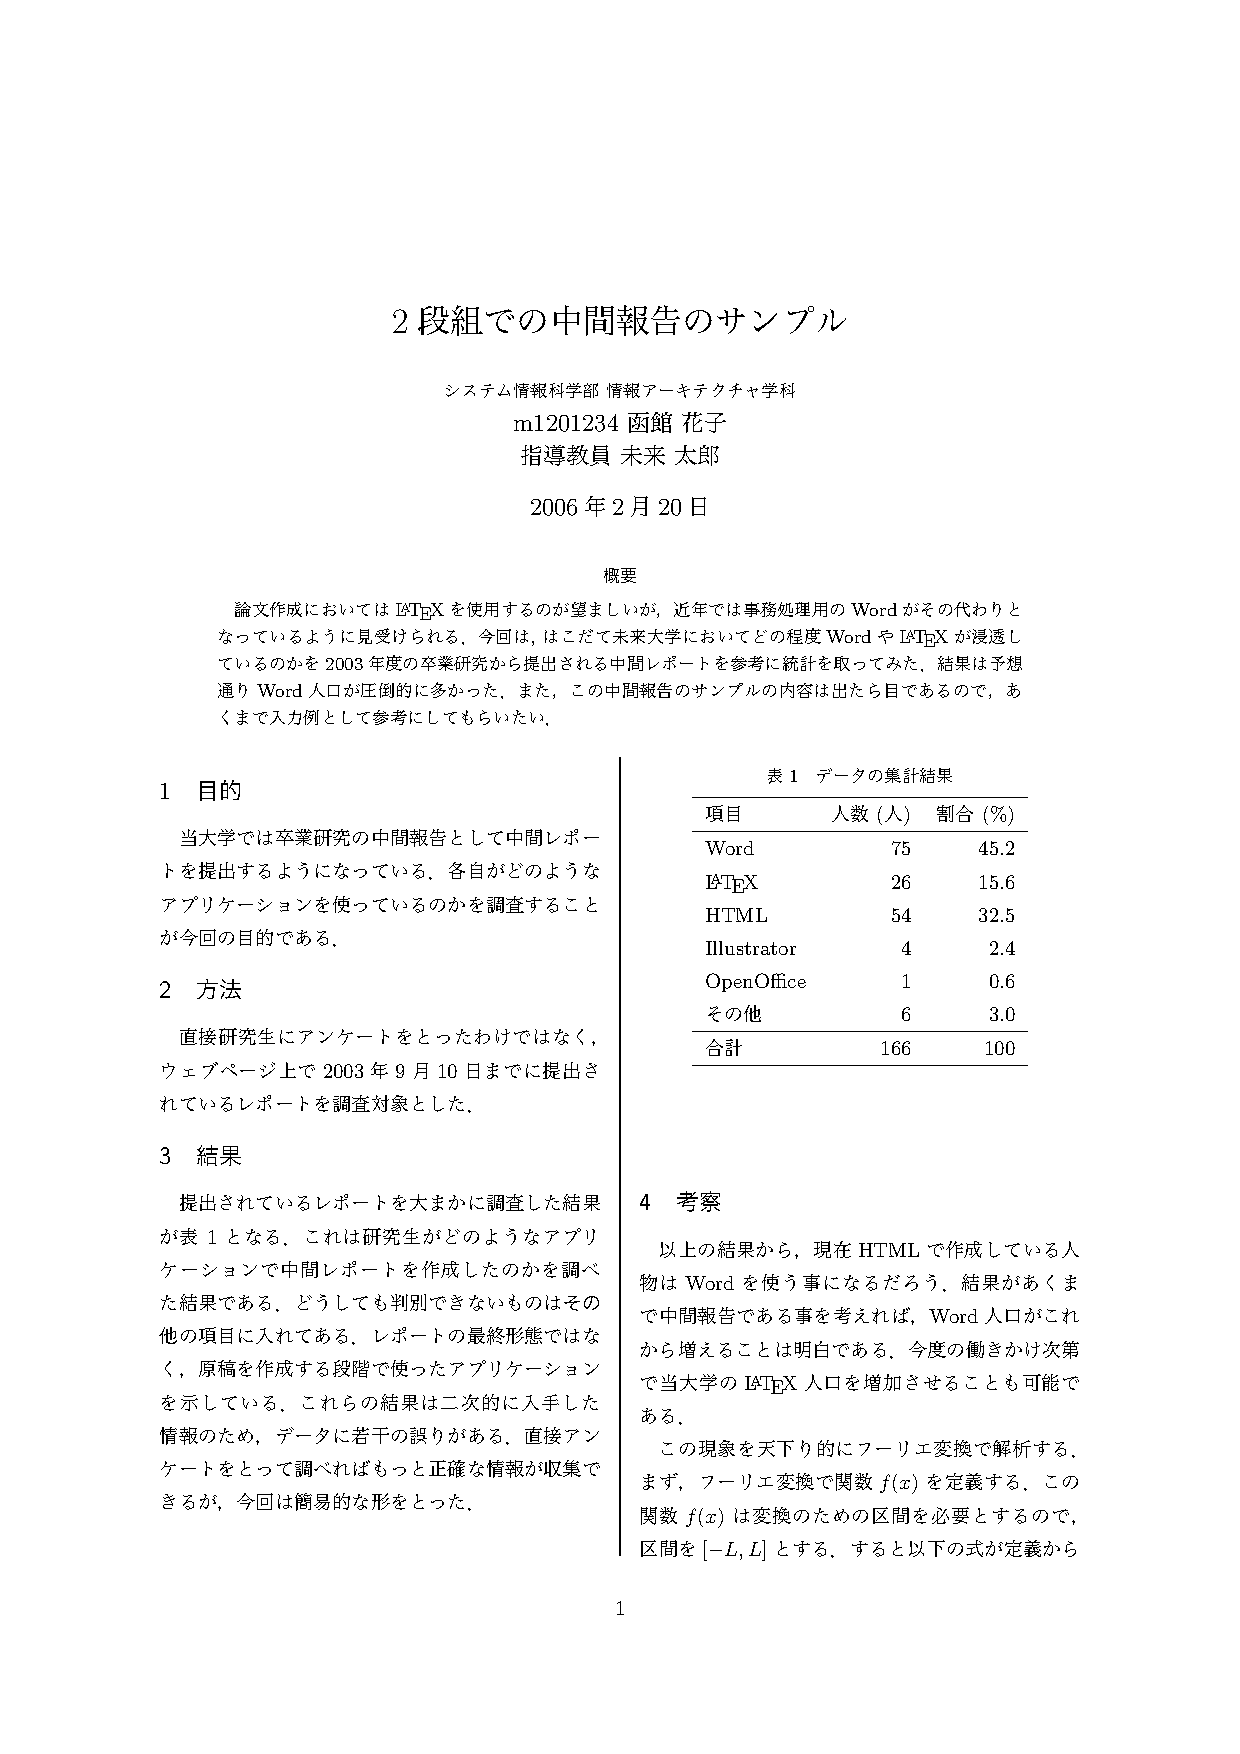
\includegraphics[width=\ftextwidth]{images/abst1}}
%\end{center}
%\clearpage
%\begin{center}
% \fbox{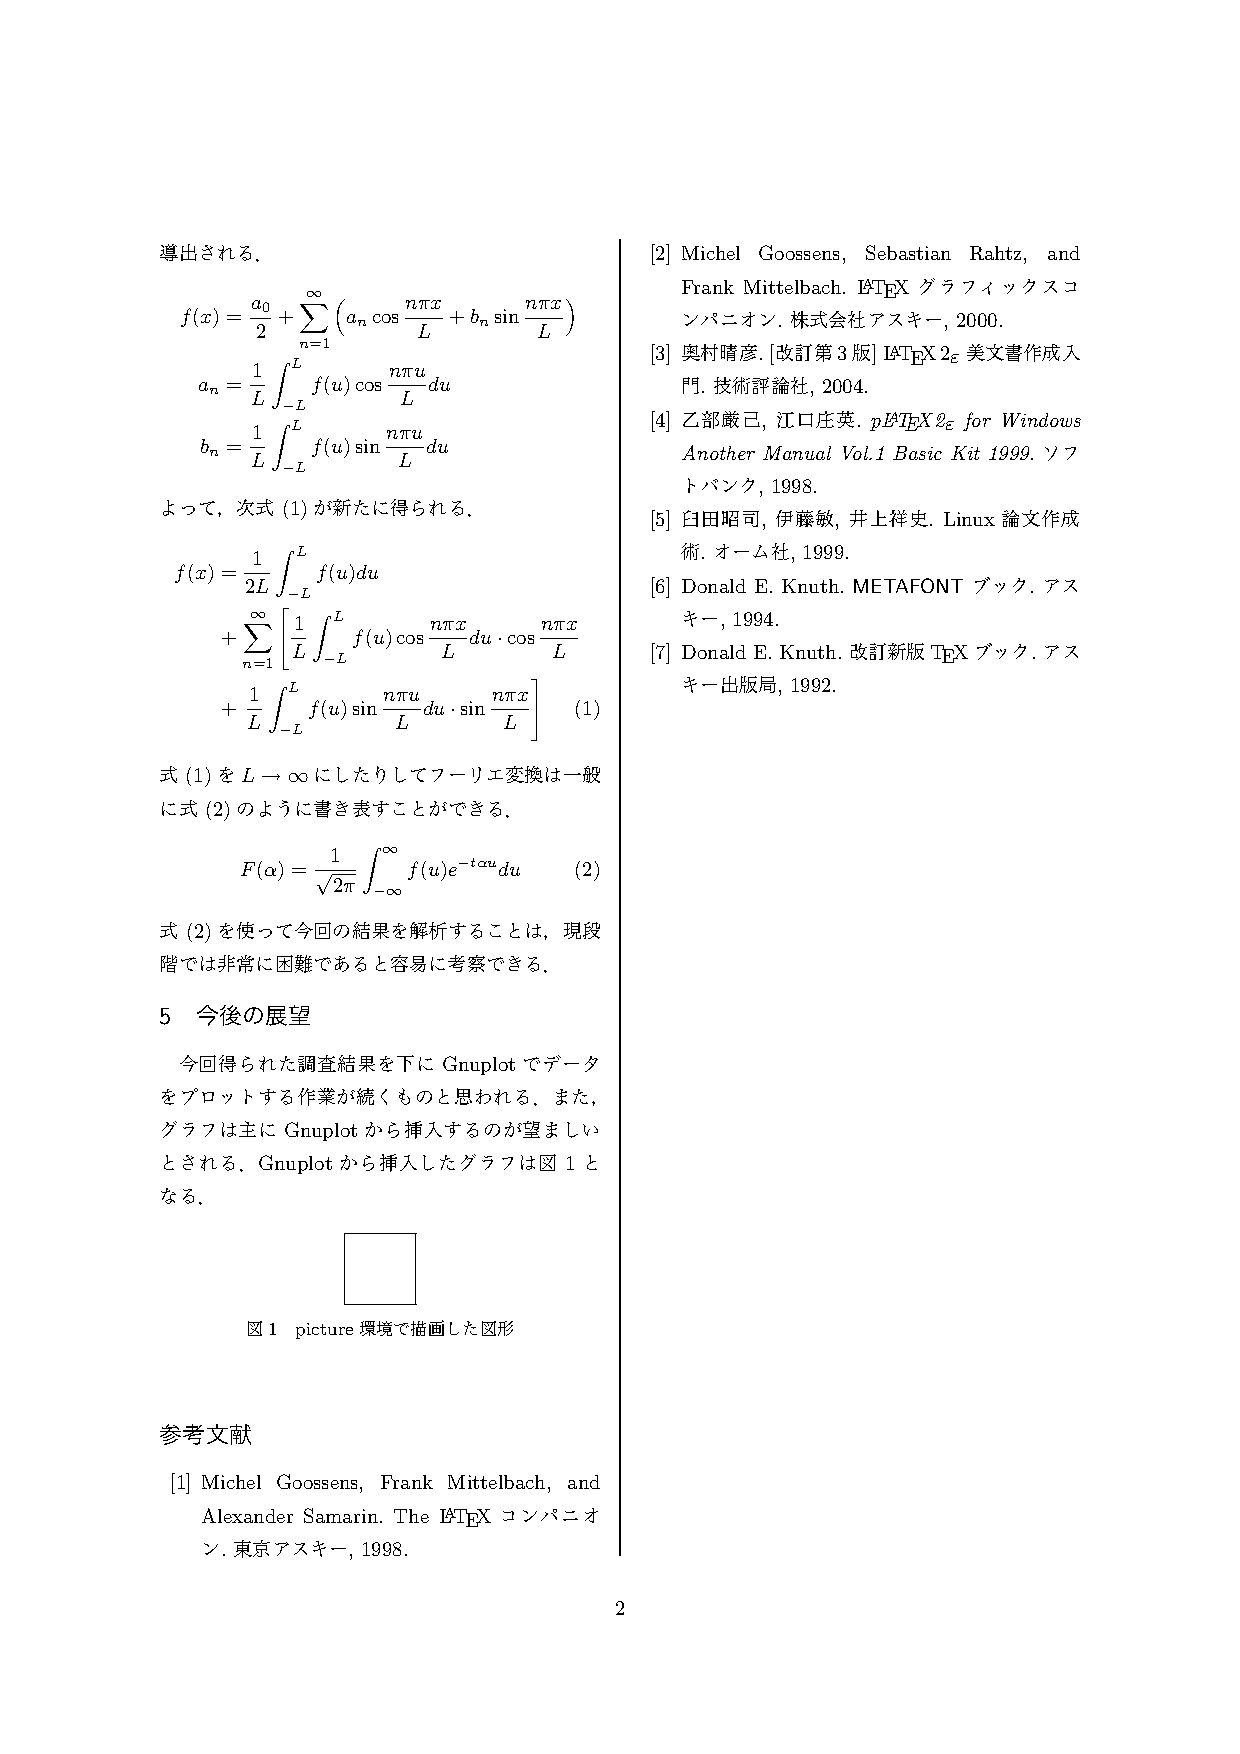
\includegraphics[width=\ftextwidth]{images/abst2}}
%\end{center}

\clearpage

\noindent \IOmargin \makebox[0pt][l]{%
\fbox{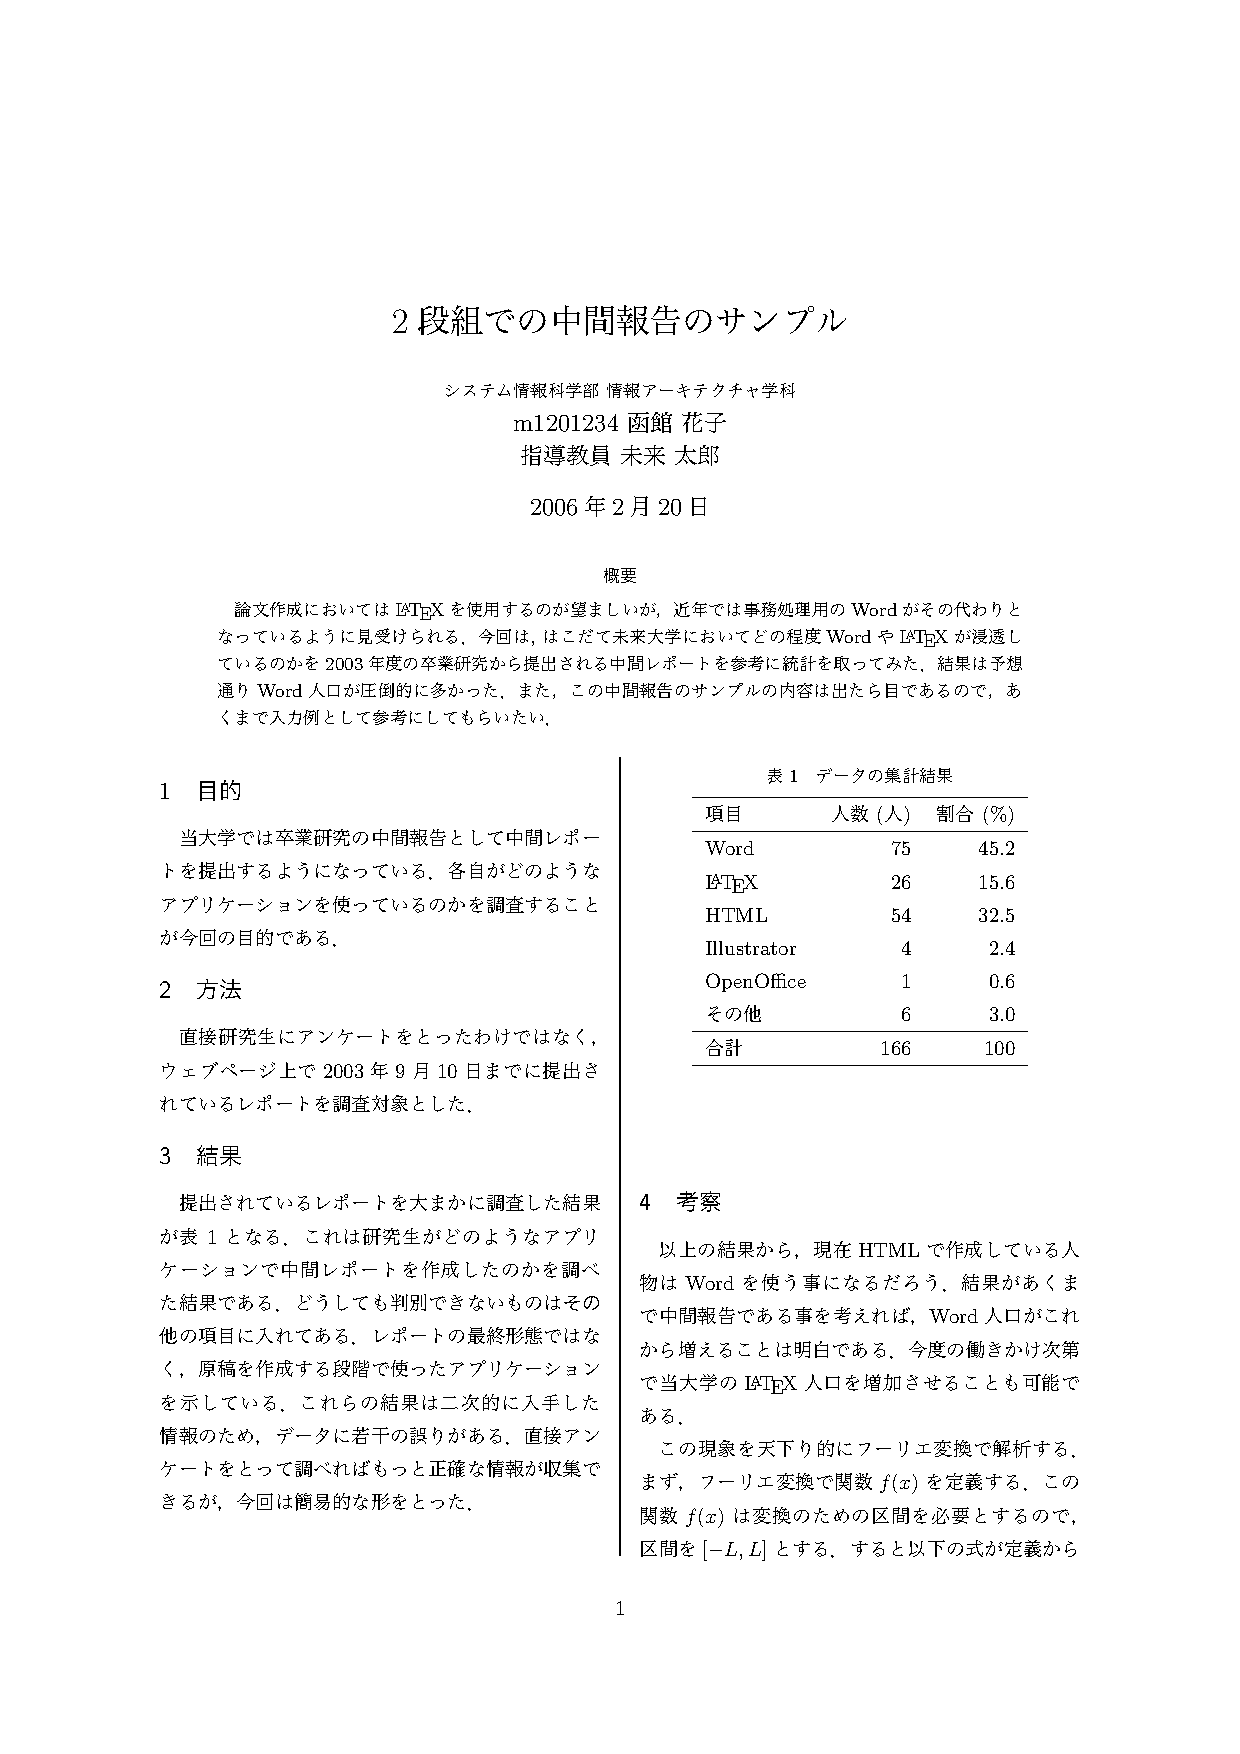
\includegraphics[clip,bb={0 0 595 842},width=\ffullwidth]
   {images/abst1}\IOlabel}}

\clearpage

\noindent \IOmargin \makebox[0pt][l]{%
\fbox{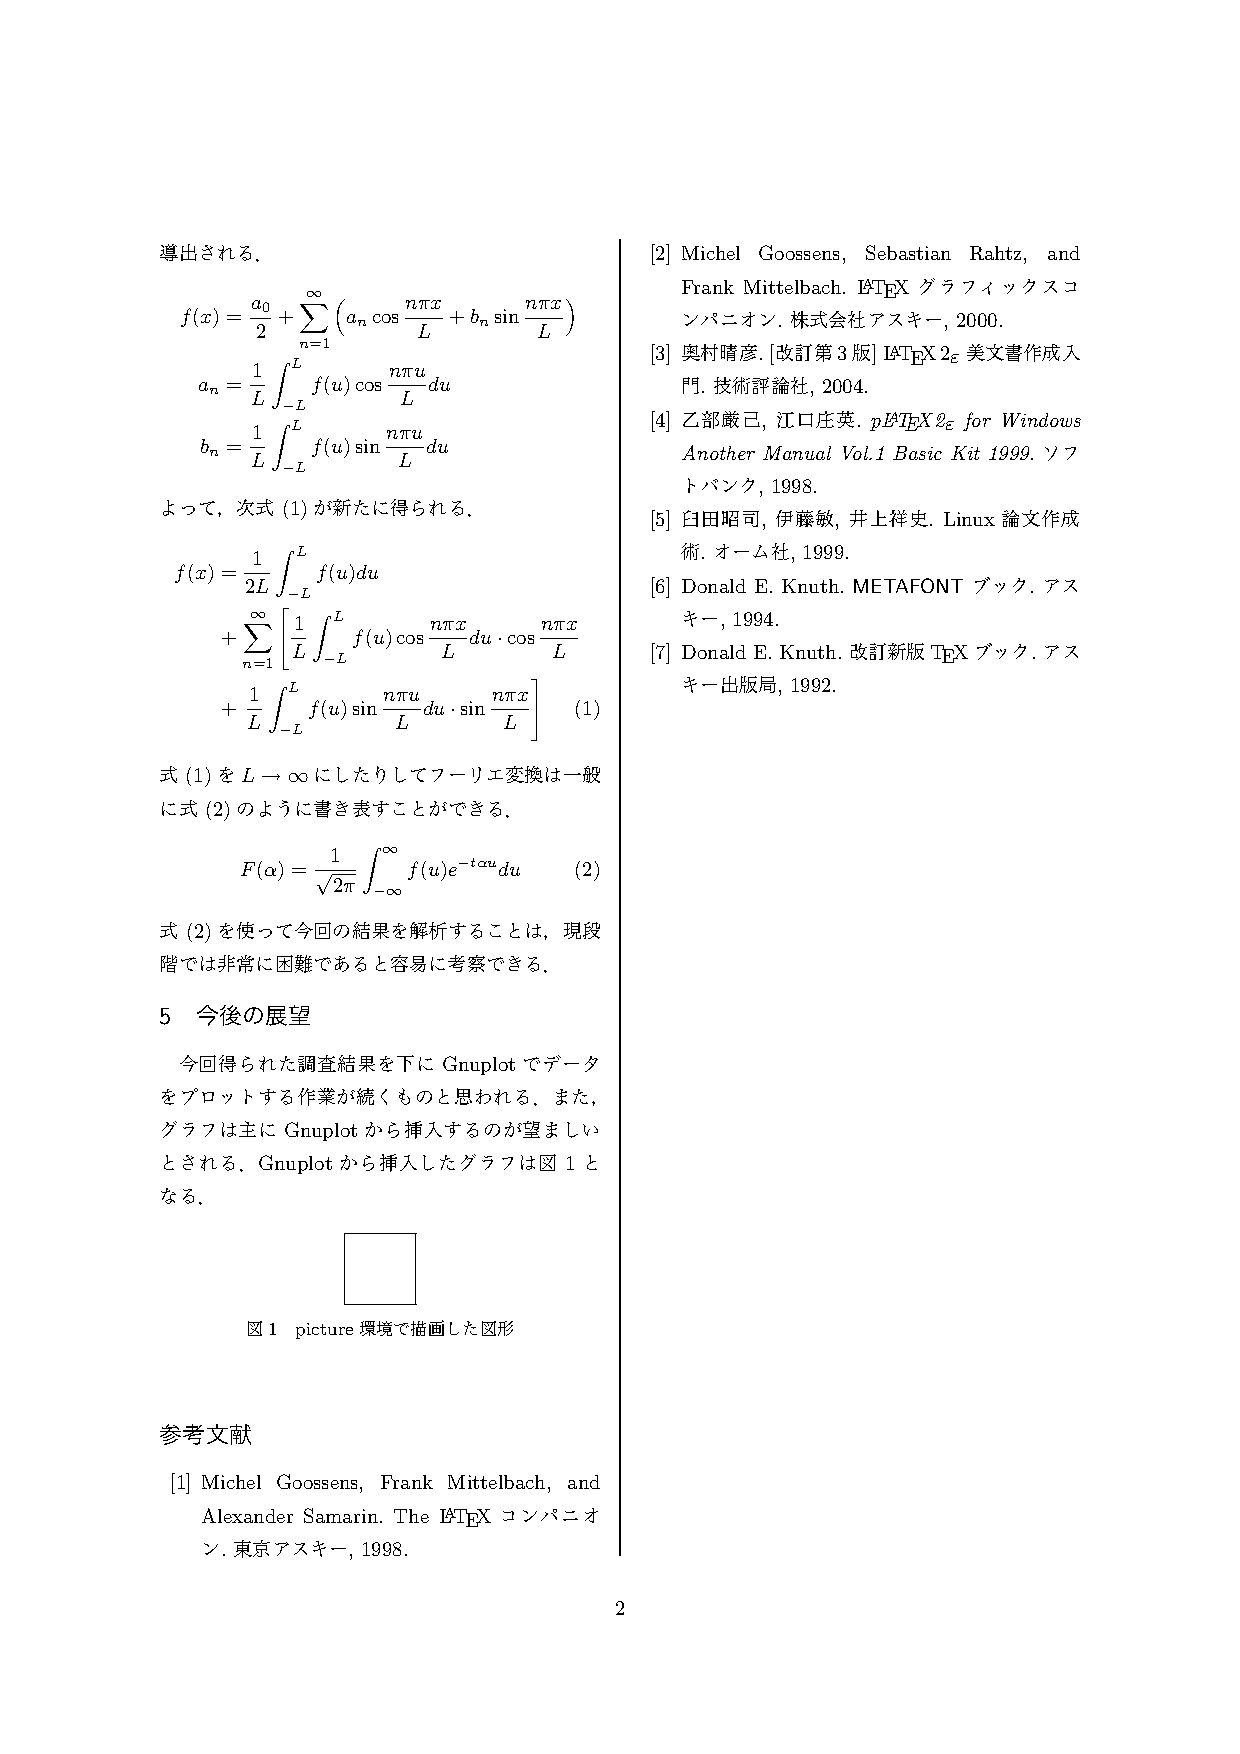
\includegraphics[clip,bb={0 0 595 842},width=\ffullwidth]
   {images/abst2}\IOlabel}}


\section{学位論文のサンプル}

学位論文などは規模として大きくなるので文書クラスは
\Cls{jreport}か\Cls{jsbook}を使う事になると思います.

\cls{jsbook}の場合にクラスオプションは
次のようにすると左右起こしをせずに片面印刷で出力されます.

\begin{InTeX}
\documentclass[11pt,report]{jsbook}
\end{InTeX}

\cls{jreport}や\cls{jsbook}で使用できる見出し
は \C{chapter},  \C{section},  \C{subsection}
の三つです.\Cmd{subsubsection}命令はなるべく使わないほう
が良いでしょう.\cls{jsarticle}文書クラスで使用できた
\env{abstract}環境は使えなくなりますので
次のようにして\Z{章立て}します.

\begin{InTeX}
\chapter*{概要}\addcontentsline{toc}{chapter}{概要}
ここに簡潔に概要を書く.
\end{InTeX}




\subsection{クラスファイルが提供されている場合}

学位論文などは大学側から文書クラスが提供される事があります.
%当大学の卒業論文の場合は\Cls{funthesis}というクラスファイル
%が配布されていますのでこれを使うことになります.
%クラスファイルとして\cls{funthesis}を使った例を示します.
%出力は省略させていただきます.

\begin{InTeX}
%\documentclass[english]{funthesis}%本文が英語のとき
\documentclass{funthesis}
\usepackage[dvipdfmx]{graphicx}%dvipsの場合は`dvips'にする
% 日本語の題名
% 長いときは`\\'で改行
\jtitle{公立はこだて未来大学における卒業論文の
{\LaTeX}クラスファイルの設計に関する考察}
% 論文の英文タイトル
\etitle{Title in English}
% 氏名(日本語)
\jauthor{未来 太郎}
% 氏名(英語)
\eauthor{Taro MIRAI}
% 所属学科名
\affiliciation{複雑系アーキテクチャ学科}
% 学籍番号
\studentnumber{1300000}
% 正指導教員名
\advisor{正指導 教員}
% 副指導教員がいる場合はコメントアウトし名前を書く
% 副指導教員がいない場合は,ここは削除しても可
%\coadvisor{副指導 教員}
% 論文提出日
\date{2004/01/31}
%ここから本文の始まり
\begin{document}
% 表紙
\maketitle
%英語の概要
\begin{eabstract} Abstract in English. (about 500 words)
\fake{you should write your English abstract in one page. }
% 英文キーワード
\begin{ekeyword}
Keyrods1, Keyword2, Keyword3, Keyword4, Keyword5
\end{ekeyword}
\end{eabstract}
% 和文概要(2000字程度)
\begin{jabstract} 日本語の概要を書く.(約200字)
\fake{ここに日本語の概要を書きます.}
% 和文キーワード
\begin{jkeyword}
キーワード1, キーワード2, キーワード3, キーワード4, キーワード5
\end{jkeyword}
\end{jabstract}
% 目次
\tableofcontents 
% 図目次
\listoffigures
% 表目次
\listoftables
\chapter{序論} % 章(chapter)のタイトル
ここに序論を書きます.
\section{背景} % 節(section)のタイトル
以下に背景,関連する環境,状況,技術に関する概要を記述.
\chapter{考察}
考察しました.
\section{評価結果}
どっこいどっこいです.
\chapter{結論と今後の展開}
どれもだめでした.
% 以降,付録(付属資料)であることを示す
\begin{appendix}
\chapter{アルゴリズム}
%付録その1(関連資料など)を必要があれば載せる
\section{あるアルゴリズム}
%付録その2(関連資料など)を必要があれば載せる
\chapter{ソースコード}
プログラムのソースコードなどを掲載します.
\section{あるソースコード}
何かを処理するあるプログラム\texttt{hoge.cpp}のプログラムを示す.
\begin{verbatim}
int main( void ){ return 0; }
\end{verbatim}
\fake[40]{{\thehoge}行\par}
%付録の終わり
\end{appendix}
\chapter*{謝辞}
謝辞を書く.
% 参考文献
\begin{thebibliography}{9}
 \bibitem{ラベル} 著者名. 書籍名. 出版社, 年号.
 \bibitem{MT1999} 未来太郎. 未来の未来. どこかの出版, 1999. 
\end{thebibliography}
\end{document}
\end{InTeX}
%

\subsection{クラスファイルが提供されていない場合}

もし大学・機関側からクラスが提供されていない場合は自前で作成する
事になります.大抵の場合はTimes系のフォントを使ってフォントサイズは何々
でという細かい指定をしてくるのが普通のようです.親切な方がすでに作成してウェ
ブで公開してくれている場合もあります.

とりあえず子供だましですが\Cls{jsbook}を用いた例を紹介します.
\cls{jreport}を使っても良いですが\cls{jsbook}の方が個人的には
良いと感じています.まずはご自分の提出・投稿先の規定に合わせて
\cls{jsbook}の定義のいくつかに変更を加えます.\cls{jsbook}
そのものに変更を加えるとどこにどのような変更を加えたのかが分か
らなくなる問題などがありますので,別ファイル\fl{mygs.sty}に変更
したマクロなどをまとめておきます.ファイルの先頭に
次のようなファイル情報を書き込んでおくと良いでしょう.

\begin{InTeX}
%% File: mygs.sty
%% Copying : Your Name
%% E-mail  : name@univ.ac.jp
%% Date    : 2006/04/20
\ProvidesPackage{mygs}[2006/04/20 First Family]
\end{InTeX}


大抵の機関では\Z{Times}系のフォントを指定すると思いますので
次の1行もあると良いでしょう.

\begin{InTeX}
\RequirePackage{txfonts}
\end{InTeX}

マクロパッケージの中で他のパッケージを
必要とする場合は \C{Requirepacakge} 命令を使います.

次にページレイアウトについてです.マージンについても細かい
指定をしてくるかもしれませんが,一定の設定方法を紹介しましょう.
ページレイアウトで設定できる項目については\figref{pagelayout}
を見てください.まずは1行の字数です.1行40文字であったとすると
長さ \Cmd{textwidth}に全角40文字の幅\pp{40zw}を指定します.

\begin{InTeX}
\setlength\textwidth{40zw}
\setlength\fullwidth{\textwidth}%jsbookで必要
\end{InTeX}

行数が40行と指定されているのであれば, \Cmd{textheight}に40\Z{行送り}
分の長さ \pp{40\Cmd{baselineskip}} を指定します.

\begin{InTeX}
\setlength\textheight{40\baselineskip}
\end{InTeX}

この程度でも良いと思うのですが,ページレイアウトの設定をしても良いでしょう.

\C*{hoffset}%
\C*{voffset}%
\C*{evensidemargin}%
\C*{oddsidemargin}%
\C*{topmargin}%
\C*{headheight}%
\C*{headsep}%
\C*{marginparwidth}%
\C*{marginparpush}%
\C*{marginparsep}%
\begin{InTeX}
\setlength\hoffset{13\p@}
\setlength\voffset{0\p@}
\setlength\evensidemargin{0\p@}
\setlength\oddsidemargin{\evensidemargin}
\setlength\topmargin{0\p@}
\setlength\headheight{0\p@}
\setlength\headsep{0\p@}
\setlength\marginparwidth{0\p@}
\setlength\marginparpush{0\p@}
\setlength\marginparsep{0\p@}
\end{InTeX}

ここでの \C{p@} は
単位\qu{pt}の事です.マクロの中ではこのような命令を使うと良
いそうです.ここでは傍注やヘッダーを出力しないと仮定して
ほとんどの項目に\qu{0pt}を代入しています.

ヘッダーやフッターは割とシンプルなもので良いと思うので
\cls{jsbook}の場合はフッターの中央にページ番号を出力するようにします.

\begin{InTeX}
\pagestyle{plainfoot}
\end{InTeX}

\cls{jreport}は最初からシンプルな\str{plain}という
ページスタイルになっています.
ただし,\qu{-- 13 --}のようにダッシュも入れるときは
次のようにします.

\zindind{太字}{のページ番号}%
\C*{footskip}%
\C*{baselineskip}%
\begin{InTeX}
 \let\@mkboth\@gobbletwo
 \let\@oddhead\@empty
 \let\@evenhead\@empty
 \def\@oddfoot{\normalfont\hfil-- \thepage\ --\hfil}%
 \let\@evenfoot\@oddfoot
 \setlength\footskip{2\baselineskip}%必要に応じて
\end{InTeX}

ページ番号を太字にするときは \C{normalfont}
の後に \Cmd{bfseries}を追加します.

%見出しのフォントの場合は和文はゴシック,欧文はTimes Bold
見出しのフォントで和文をゴシック,欧文はTimes Boldにしたいとき,
\cls{jsbook}の場合は次のようにしておけば良いでしょう.

\begin{InTeX}
\renewcommand{\headfont}{\gtfamily\rmfamily\bfseries}
\end{InTeX}

\cls{jsbook}は標準で
は欧文がサンセリフ体になっています.\cls{jreport}の場合
は最初から欧文がボールド体に設定されています.

おまけに目次の深さを決めるカウンタ\str{tocdepth}も
次のようにすると \C{subsection} まで出力されます.

\begin{InTeX}
\setcounter{tocdepth}{2}
\end{InTeX}


\cls{jreport}の場合は見出しの後の字下げが行われない事がありますので次
のようにして\Sty{indentfirst}パッケージを読み込みます.

\begin{InTeX}
\RequirePackage{indentfirst} 
\end{InTeX}


これらをまとめると自分のマクロパッケージ\sty{mygs.sty}が
出来上がりです\footnote{\url{http://tex.dante.jp/jou1/mygs.sty}}.

\begin{InTeX}
%% File: mygs.sty
%% Copying : Thor Watanabe
%% E-mail  : thor@tex.dante.jp
%% Date    : 2006/04/20
\ProvidesPackage{mygs}[2006/04/20 First Family]
\RequirePackage{txfonts}% Times系のフォントを使う
%\RequirePackage{indentfirst}% jreportは必要
\setlength\textwidth{40zw}%1行40文字
\setlength\fullwidth{\textwidth}%jsbookでは必要
\setlength\textheight{40\baselineskip}%1ページ40行
\setlength\hoffset{13\p@}%\p@は0ptのこと
\setlength\voffset{0\p@}
\setlength\evensidemargin{0\p@}
\setlength\oddsidemargin{\evensidemargin}
\setlength\topmargin{0\p@}
\setlength\headheight{0\p@}
\setlength\headsep{0\p@}
\setlength\marginparwidth{0\p@}
\setlength\marginparpush{0\p@}
\setlength\marginparsep{0\p@}
\setlength\footskip{2\baselineskip}%必要に応じて
\def\ps@foot{%フッターに `-- ページ番号 --'としたいとき
 \let\@mkboth\@gobbletwo
 \let\@oddhead\@empty
 \let\@evenhead\@empty
 \def\@oddfoot{\normalfont\hfil-- \thepage\ --\hfil}%
 \let\@evenfoot\@oddfoot
}
\pagestyle{plainfoot}%jsbookならば
%\pagestyle{plain}%jreportならば
\renewcommand{\headfont}{\normalfont\bfseries}
\setcounter{tocdepth}{2}
\end{InTeX}

そのような作業が終わったら自分の論文の主となるソースファイル
を書き上げます.用紙はA4で,フォントサイズは11\,pt,左右起こし
はせずに片面印刷というのが一般的だと思いますから次のようにします.

\begin{InTeX}
\documentclass[a4j,11pt,report]{jsbook}
\end{InTeX}

そして先程作成した\fl{mygs.sty}を \C{usepackage}命令で読み込みます.

\begin{InTeX}
\usepackage{mygs}
\end{InTeX}


この程度でも良いのですが,表紙もまた細かい指定をされる場合
があります.1から \cmd{maketitle}を作っても良いのですが,一
刻も早く論文を仕上げなければならないときに,命令を定義して
は間に合わないかも知れません.そのようなときは断腸の思い
で \Cmd{titlepage}環境を借用して表紙を作る事もできます.%
\indindz{表題}{表紙の}\index{表紙の作成}%
例として \Cmd{maketitle}命令の変更例を紹介します.

\C*{vskip}%
\C*{cvs}%
\C*{headfont}%
\C*{null}%
\begin{InTeX}
\renewcommand{\maketitle}{%
\begin{titlepage}
    \let\footnotesize\small
    \let\footnoterule\relax
    \let\footnote\thanks
    \null\vskip2\cvs%ページ上部の空白
    \begin{center}\thispagestyle{empty}%
      {\LARGE\headfont ここに表題を書きます}\par\vskip\cvs
      {\Large\normalfont 未来太郎}\par\vskip2\cvs
      {\small 未来研究学科 \qquad 学籍番号}\par\vskip.5\cvs
      {\small 指導教員 \qquad 北海太郎}\par\vskip2\cvs
      {提出日 2006/03/30}\par\vskip3\cvs
      {\Large\headfont English Title}\par\vskip\cvs
      {\large\rmfamily Your Name}\par\vskip\cvs
    \end{center}%
    \vfill\null
\end{titlepage}}
\end{InTeX}

\C{vskip}とは垂直方向に空きを挿入する命令です.

以上は例ですので先方に規定された通りのレイアウトに
適宜変更してください.



見出しを出力する \cmd{section} 命令の体裁が適切ではないと
思われるのであれば,適宜 \cmd{section}型の命令を再定義します.

\begin{Syntax}
\C{@startsection}\pa{見出しの種類}%
  \pa{階層}\pa{字下げ}\pa{前空き}\pa{後空き}\\
\hskip3zw\pa{体裁}\str*\opa{目次用の見出し}\pa{見出し}
\end{Syntax}

\begin{Exe}
実際に \fl{jsbook.cls}から \cmd{section}の定義を何かしらのファイルにコピー
してください.

\begin{InTeX}
\makeatletter
\renewcommand{\section}{%
    \if@slide\clearpage\fi
    \@startsection{section}{1}{\z@}%
    {\Cvs \@plus.5\Cdp \@minus.2\Cdp}% 前アキ
    {.5\Cvs \@plus.3\Cdp}% 後アキ
    {\normalfont\Large\headfont\raggedright}}
\makeatother 
\end{InTeX}

\cmd{newcommand} は \cmd{renewcommand} に変更します.
ここで,\Cmd{raggedright}となっている箇所を \Cmd{centering}
等に変更すると結果はどのようになるか吟味してください.
\end{Exe}

他にも章見出しの体裁は \C{@makechapterhead}, \C{@makeschapterhead},
図表見出しの体裁は \C{@makecaption},文献一覧のラベルの体裁
は \C{@biblabel}という具合に,それぞれ対応するコマンドが存在します.

\begin{Prob}
次の記述を追加すると \C{section}等の命令はどのように変わるでしょうか.

\begin{InTeX}
\renewcommand\@seccntformat[1]{\@nameuse{the#1}.\quad}
\end{InTeX}

実際にタイプセットし,出力結果を吟味してください.
% 単に見出しの最後にピリオドが付きます.
\end{Prob}

\begin{Prob}
章見出しは実際に \C{@makechapterhead} 命令で表示されます.
7行目の`\cmd{par}\C{nobreak}'と`\C{vskip} \C{Cvs}'という記述を削除する
とどうなりますか?
また,\cmd{raggedright}を \cmd{centering}等に変更するとどのような
出力結果になるのか,実際にタイプセットして確認してください.

\begin{InTeX}
\def\@makechapterhead#1{%
  \vspace*{2\Cvs}% 欧文は50pt
  {\parindent \z@ \raggedright \normalfont
    \ifnum \c@secnumdepth >\m@ne
      \if@mainmatter
        \huge\headfont \@chapapp\thechapter\@chappos
        \par\nobreak
        \vskip \Cvs % 欧文は20pt
      \fi
    \fi
    \interlinepenalty\@M
    \Huge \headfont #1\par\nobreak
    \vskip 3\Cvs}} % 欧文は40pt
\end{InTeX}

\end{Prob}

\begin{Prob}
\cls{jsclasses}の\env{quotation}環境では,右余白が 0\,ptに設定
されています.それでは \env{quotation}環境を下記のように再定義すると,
結果はどのようになるのか,実際にタイプセットして確認してください.

\begin{InTeX}
\renewenvironment{quotation}{%
  \list{}{%
    \listparindent\parindent
    \itemindent\listparindent
    \rightmargin = \leftmargin}%
  \item\relax}{\endlist}
\end{InTeX}
\end{Prob}

\begin{Prob}
図表見出しは \C{@makecaption} によって表示されています.
では,`\verb|\advance\leftskip1cm|'と`\verb|\advance\rightskip1cm|'という
記述を削除すると結果はどうなるか,実際にタイプセットして確認してください.

\begin{InTeX}
\long\def\@makecaption#1#2{{\small
  \advance\leftskip1cm
  \advance\rightskip1cm
  \vskip\abovecaptionskip
  \sbox\@tempboxa{#1\hskip1zw\relax #2}%
  \ifdim \wd\@tempboxa <\hsize \centering \fi
  #1\hskip1zw\relax #2\par
  \vskip\belowcaptionskip}} 
\end{InTeX}
\end{Prob}

\begin{Prob}
目次中における章見出しは \C{l@chapter}で表示されます.
では \C{begingroup}の後に \C{large}を記述するとどうなるか,
実際にタイプセットし,それを確認してください.

\begin{InTeX}
\renewcommand*{\l@chapter}[2]{%
  \ifnum \c@tocdepth >\m@ne
    \addpenalty{-\@highpenalty}%
    \addvspace{1.0em \@plus\p@}
    \begingroup
      \parindent\z@
      \rightskip\@tocrmarg
      \parfillskip-\rightskip
      \leavevmode \large \headfont % ここに \large を追加
      \setlength\@lnumwidth{4.683zw}%
      \advance\leftskip\@lnumwidth \hskip-\leftskip
      #1\nobreak\hfil\nobreak\hbox to\@pnumwidth{\hss#2}\par
      \penalty\@highpenalty
    \endgroup
  \fi} 
\end{InTeX}
\end{Prob}



%\begin{table}[htbp]
% \begin{center}
%  \caption{各種学会の論文投稿用クラス・マクロ}\tablab{gakkai}
% \begin{tabular}{ll}
% \egakkai{IEEE}
% \gakkai{映像情報メディア}
% \gakkai{計測自動制御}
% \gakkai{言語処理}
% \gakkai{システム制御情報}
% \gakkai{人工知能}
% \gakkai{精密工}
% \gakkai{電気}
% \gakkai{電子情報通信}
% \gakkai{ヒューマンインタフェース}
% \gakkai{日本音響}
% \gakkai{日本計測工}
% \gakkai{日本機会}
% \gakkai{日本ソフトウェア科}
% \gakkai{日本ロボット}
% \gakkai{日本オペレーションズリサーチ}
% \gakkai{土木学会}
% \gakkai{日本信頼性}
% \gakkai{日本数式処理}
% \gakkai{日本統計}
% \gakkai{プラズマ/核融合}
% \gakkai{日本神経回路}
% \end{tabular}
% \end{center}
%\end{table}

